\documentclass[12pt,a4paper]{article}

% Margins.
\setlength{\oddsidemargin}{0in}
\setlength{\evensidemargin}{0in}
\setlength{\headheight}{12pt}
\setlength{\headsep}{42pt}
\setlength{\topmargin}{-74pt}
\setlength{\textwidth}{6.5in}
\setlength{\textheight}{10in}
\pagestyle{plain}

\usepackage{amsmath}
\usepackage{float}
\usepackage{graphicx}
\usepackage[hyphens]{url}
\usepackage[hidelinks]{hyperref}	% Clickable links to figures, references and urls.
\usepackage{lastpage}

% Drawing.
\usepackage{pgf}
\usepackage{tikz}

% Listings for formatting code.
\usepackage{listings}
\usepackage{textcomp}
% General options.
\lstset{breaklines=true, basicstyle=\footnotesize\ttfamily, tabsize=4, numbers=none, stepnumber=1, frame=single, showstringspaces=false, upquote=true}
% C++ specific high-lighting. Comments are 50/50 shades of green/black and strings coloured with 60/40 red/black mixture.
\lstset{language=[ISO]C++, commentstyle=\color{green!50!black}, keywordstyle=\color{blue}, stringstyle=\color{red!60!black}}

% Marks of each question.
\def\QOne{10}
\def\Qtwo{10}
\def\Qthree{10}
\def\Qfour{10}
\def\Qfive{10}
\def\Qsix{10}
\def\Qseven{10}
\def\Qeight{10}
\def\Qnine{10}
\def\Qten{10}
\def\TotalMarks{100}

\begin{document}
\begin{minipage}{0.55\textwidth}
{\LARGE \textbf{Physics for Engineers}}\\[0.15cm]
{\normalsize \textbf{Fall 2013 Semester}}\\
{\Large \textbf{Final Exam}}\\
{\normalsize \textbf{Monday, December 16, 2013}}\\[0.30cm]
{\Large \textbf{Total Time: 180 minutes}}\\[0.15cm]
{\Large \textbf{Total Marks: 100}}\\
\textbf{Course Instructors:}\\
Arshad Hassan\\
Attique Dawood\\
\end{minipage}
\begin{minipage}{0.4\textwidth}
\textbf{Serial} \hrulefill \\[0.25cm]
\textbf{Name} \hrulefill\\[0.25cm]
\textbf{Section} \rule{1cm}{0.2mm} \textbf{Roll No:} \hrulefill\\[0.25cm]
\textbf{Signature:} \hrulefill\\[0.25cm]
\rule{6.6cm}{0.2mm}\\
\textbf{Signature of Invigilator}\\[0.25cm]
\end{minipage}
\begin{table}[H]
\begin{center}
\vspace{0.3cm}
	{\large \begin{tabular}{|l|c|c|c|c|c|c|c|c|c|c|c|}
	\hline
		\rule{0pt}{2.6ex} Question & \textbf{1} & \textbf{2} & \textbf{3} & \textbf{4} & \textbf{5} & \textbf{6} & \textbf{7} & \textbf{8} & \textbf{9} & \textbf{10} & \textbf{Total}\\
		\hline
		Total Marks \rule{0pt}{2.6ex} & \QOne & \Qtwo & \Qthree & \Qfour & \Qfive & \Qsix & \Qseven & \Qeight & \Qnine & \Qten & \TotalMarks\\
		\hline
		Marks Obtained \rule{0pt}{2.6ex} & & & & & & & & & & &\\
	\hline
	\end{tabular}}
\end{center}
\end{table}
\noindent \textbf{You are advised to READ these notes:}
\begin{enumerate}
\item \textbf{Attempt on the Question Paper. \underline{NO EXTRA SHEET} will be provided/accepted. No
additional sheet will be provided for rough work. Use the back of the page where
provided space is not sufficient.}
\item After asked to commence the exam, please verify that you have \textbf{\pageref{LastPage} different
printed pages} including this title page.
\item There are 5 questions. Attempt all of them. It is advisable to go through the paper once
before starting with the first question.
\item Exam is closed books, closed notes. Please see that the area in your threshold is clean.
You will be charged for any material which can be classified as \textbf{`helping in the paper'}
found near you.
\item All distances and coordinates are in meters.
\item \textbf{Calculator sharing is strictly prohibited.}
\item Students who attempt the paper with lead pencils lose the right to get them rechecked.
\item \textbf{The invigilator present is not supposed to answer any questions. No one may come
to your room for corrections and you are not supposed to request to call anyone.
Make assumptions wherever required and clearly mark them.}
\end{enumerate}
\newpage
\noindent\textbf{Question 1: Line Integral\hfill \QOne~marks}\\
Given a vector field $\textbf{A}=2y\hat x+2xy\hat y$ find the circulation of \textbf{A} ($\oint\limits_{L} \textbf{A}\cdot d\textbf{\textit{l}}$) over closed path ABCDA.
\begin{figure}[H]
\flushright
\begin{tikzpicture}[xscale=1.2,yscale=1.2,font=\small]
	\def\XD{0cm}
	\def\YD{0cm}

	\draw[thick, ->, >=stealth] (1cm, 2cm) -- (3cm, 2cm);
	\draw[thick, ->, >=stealth] (3cm, 2cm) -- (3cm, 4cm);
	\draw[thick, ->, >=stealth] (3cm, 4cm) -- (1cm, 4cm);
	\draw[thick, ->, >=stealth] (1cm, 4cm) -- (1cm, 2cm);
	%\draw[thick, ->, >=stealth] (2cm, 4cm) -- (1cm, 2cm);

	%\draw[dashed] (0cm, 0cm) -- (1cm, 2cm);
	\draw[dashed] (0cm, 2cm) -- (1cm, 2cm);
	\draw[dashed] (0cm, 4cm) -- (1cm, 4cm);
	\draw[dashed] (1cm, 0cm) -- (1cm, 1.6cm);
	\draw[dashed] (3cm, 0cm) -- (3cm, 1.6cm);
	%\draw[white,fill=white] (0.5cm,0.5cm) rectangle (1.5cm, 0.9cm);
	%\node at (1cm, 0.7cm){$y=2x$};

	\coordinate[label=above:$C$] (C) at (3cm,4cm);
	\coordinate[label=above:$D$] (D) at (1cm,4cm);
	\coordinate[label=below:$A$] (A) at (1cm,2cm);
	\coordinate[label=below:$B$] (B) at (3cm,2cm);
	
	\coordinate[label=left:$2$] (y1) at (0cm,2cm);
	\coordinate[label=left:$4$] (y2) at (0cm,4cm);
	\coordinate[label=below:$1$] (x1) at (1cm,0cm);
	\coordinate[label=below:$3$] (x2) at (3cm,0cm);
	
	\draw[thick, ->, >=stealth] (0cm, 0cm) -- (0cm, 5cm);
	\coordinate[label=above:$y$] (y) at (0cm,5cm);
	\draw[thick, ->, >=stealth] (0cm, 0cm) -- (4cm, 0cm);
	\coordinate[label=right:$x$] (x) at (4cm,0cm);

\end{tikzpicture}
\end{figure}
\vspace{-8.2cm}
\begin{figure}[H]
\begin{tikzpicture}
	\draw[thick] (0cm,0cm) rectangle (\textwidth, 23cm);
\end{tikzpicture}
\end{figure}

\noindent \textbf{Question 2: Surface Integral\hfill \Qtwo~marks}\\
In a certain region $\textbf{J}=3r^2\cos\theta\hat r -r^2\sin\theta\hat\theta$ A/m$^2$. Find the current crossing the surface defined by $\theta=30^0$, $0<\phi<2\pi$ and $0<r<2$.\\
\textbf{Hint: } $I=\int\limits_{S} \textbf{J}\cdot d\textbf{S}$
\begin{figure}[H]
\begin{tikzpicture}
	\draw[thick] (0cm,0cm) rectangle (\textwidth, 22cm);
\end{tikzpicture}
\end{figure}

\noindent \textbf{Question 3: Volume Integral\hfill \Qthree~marks}\\
Volume charge density in the region $0<x<1$, $0<y<2$ and $0<z<1$ is $\rho_V=(1+xz)$ C/m$^3$. Find the total charge.
\begin{figure}[H]
\begin{tikzpicture}
	\draw[thick] (0cm,0cm) rectangle (\textwidth, 23cm);
\end{tikzpicture}
\end{figure}

\noindent\textbf{Question 4: Coulomb's Law and Electric Field \hfill \Qfour~marks}\\
Charges $q_1=1$ nC and $q_2=2$ nC are located at (0, 0, 0) and (0, 1, 0). Find electric field at (1, -2, 1).
\begin{figure}[H]
\begin{tikzpicture}
	\draw[thick] (0cm,0cm) rectangle (\textwidth, 23cm);
\end{tikzpicture}
\end{figure}

\noindent\textbf{Question 5: Electric Field of Continuous Charge Distribution\hfill \Qfive~marks}\\
A line charge is placed on $y$--axis at $0<y<5$ with uniform line charge density $\rho_L=4\pi\epsilon_0$ C/m. Calculate electric field at a point (1, 0, 0) on $x$--axis.\\
\textbf{Note:} $\int\dfrac{dx}{(x^2+a^2)^{(3/2)}}=\dfrac{x/a^2}{\sqrt{x^2+a^2}}$.
\begin{figure}[H]
\begin{tikzpicture}
	\draw[thick] (0cm,0cm) rectangle (\textwidth, 22cm);
\end{tikzpicture}
\end{figure}

\noindent\textbf{Question 6: Gauss's Law \hfill \Qsix~marks}\\
A spherical charge distribution with volume charge density $\rho_v=\dfrac{1}{4\pi r^2}$ C/m$^3$ exists in the region $r<1$. This spherical charge distribution is enclosed in a conducting shell from $r=2$ to $r=3$. Surface charge density on the outer surface of conductor was found to be $\rho_S=-\dfrac{1}{36\pi}$ C/m$^2$. Find electric field \textbf{everywhere}.
\begin{figure}[H]
\begin{tikzpicture}
	\draw[thick] (0cm,0cm) rectangle (\textwidth, 21.5cm);
\end{tikzpicture}
\end{figure}

\noindent\textbf{Question 7: Biot--Savart Law \hfill \Qseven~marks}\\
Find \textbf{H} at origin due to wire segment AB shown in figure. Current in the wire is 1 A.
\begin{equation*}
\textbf{H}=\dfrac{Ir_{12}}{4\pi|(\textbf{r}-\textbf{r}_1)\times\textbf{r}_{12}|}\left(\dfrac{(\textbf{r}-\textbf{r}_2)\cdot\textbf{r}_{12}}{|\textbf{r}-\textbf{r}_2|r_{12}}-\dfrac{(\textbf{r}-\textbf{r}_1)\cdot\textbf{r}_{12}}{|\textbf{r}-\textbf{r}_1|r_{12}}\right)\dfrac{(\textbf{r}-\textbf{r}_1)\times\textbf{r}_{12}}{|(\textbf{r}-\textbf{r}_1)\times \textbf{r}_{12}|}.
\end{equation*}
\begin{figure}[H]
\flushright
\begin{tikzpicture}[xscale=1.2,yscale=1.2,font=\small]
	\def\XD{0cm}
	\def\YD{0cm}

	% Drawing vertical grid lines.
	\foreach \x in {-2cm,-1cm,0cm,1cm,2cm}
		\draw[dashed] (\x,-2cm) -- (\x,2cm); % Solid lines at +1 intervals.
	\foreach \x/\xlabel in {-2cm/$-2$,-1cm/$-1$,1cm/$1$,2cm/$2$}
		\coordinate[label=left:\xlabel] (XLabel) at (\x,0.2cm);
	% Drawing horizontal grid lines.
	\foreach \y in {-2cm,-1cm,0cm,1cm,2cm}
		\draw[dashed] (-2cm,\y) -- (2cm,\y); % Solid lines at +1 intervals.
	\foreach \y/\ylabel in {-2cm/$-2$,-1cm/$-1$,1cm/$1$,2cm/$2$}
		\coordinate[label=left:\ylabel] (YLabel) at (0cm,\y+0.2cm);
	
	\draw[thick, ->, >=stealth] (2cm, -1cm) -- (0cm, 2cm);
	%\draw[thick, ->, >=stealth] (-1cm, 1cm) -- (2cm, 1cm);
	%\draw[thick, ->, >=stealth] (2cm, 1cm) -- (2cm, -2cm);

	\coordinate[label=below:A] (A) at (2.2cm,-1cm);
	\coordinate[label=above:B] (B) at (0.2cm,2cm);
	%\coordinate[label=above:C] (C) at (2.2cm,1cm);
	
	\draw[thick, <->, >=stealth] (0cm, -3cm) -- (0cm, 3cm);
	\coordinate[label=above:$y$] (y) at (0cm,3cm);
	\draw[thick, <->, >=stealth] (-3cm, 0cm) -- (3cm, 0cm);
	\coordinate[label=right:$x$] (x) at (3cm,0cm);

\end{tikzpicture}
\end{figure}
\vspace{-8.8cm}
\begin{figure}[H]
\begin{tikzpicture}
	\draw[thick] (0cm,0cm) rectangle (\textwidth, 22.25cm);
\end{tikzpicture}
\end{figure}

\noindent\textbf{Question 8: Ampere's Law \hfill \Qeight~marks}\\
Current density in a straight wire of radius 1 mm is $\textbf{J}=\dfrac{1}{2\pi\rho}\times 10^3$ A/m$^2$. Find \textbf{H}--field everywhere.\\
\begin{figure}[H]
\begin{tikzpicture}
	\draw[thick] (0cm,0cm) rectangle (\textwidth, 22.25cm);
\end{tikzpicture}
\end{figure}

\noindent\textbf{Question 9: Displacement Current \hfill \Qnine~marks}\\
A parallel--plate capacitor with plate area of 15 cm$^2$ has an electric field $\textbf{E}=15\sin 500t$ V/m applied across its plates. If the capacitor dielectric is $\epsilon=2.5\epsilon_0$ find the displacement current flowing through the capacitor.
\begin{figure}[H]
\begin{tikzpicture}
	\draw[thick] (0cm,0cm) rectangle (\textwidth, 22.25cm);
\end{tikzpicture}
\end{figure}

\noindent\textbf{Question 10: Maxwell's Equations \hfill \Qten~marks}\\
Write Maxwell's equations in their final form.
\begin{figure}[H]
\begin{tikzpicture}
	\draw[thick] (0cm,0cm) rectangle (\textwidth, 22.25cm);
\end{tikzpicture}
\end{figure}

\end{document}